% figures/fig4_calibration.tex -- float wrapper for Figure 4 (Sec. 5.4).
% Image produced by figures/fig4_calibration.py, which also writes
% figures/out/fig4_calibration_data.json recording every plotted number and the
% file it came from.
%
% REVISION C6 (correctness fix, applied 2026-08-14)
%   The previous version overlaid the continuous curve NRV = 1 - r^2 on a plane
%   whose points are (mean-over-parents r, median-over-parents NRV).  That curve
%   is not a valid boundary for such an aggregate: the identity is per parent,
%   NRV_min(m) = 1 - r_m^2, and mean_m[1 - r_m^2] != 1 - (mean_m r_m)^2.  The
%   curve has been REMOVED.  The optimally rescaled bound is now reported the
%   only way it can be reported honestly, as its own per-seed aggregate, in the
%   new panel (b).  The generator asserts the per-parent identity at build time.
%   The teacher point is now labelled the TEACHER-EVALUATOR AGREEMENT REFERENCE
%   (the independent evaluator scoring the training teacher), never a ceiling.
%
% PROVENANCE (every number machine-read; nothing transcribed from prose or PDF)
%   all panels  figures/out/scale_primary.json, ["dropref"][arm]["per_seed"]
%               [seed]["primary_93"].  Panel (a) uses "pearson_r" (MEAN over the
%               93 parents) and "nrv" (MEDIAN over parents); panel (b) uses
%               "nrv" and "nrv_min" (MEAN over parents); panel (c) uses
%               "T_eff_eV" (kT divided by the median per-parent slope).
%               All four are cross-checked at build time against the per-parent
%               blocks of runs/eval_ours/calibration/calibration_dropref.json
%               restricted to the 93 ids in figures/out/primary_endpoint.json;
%               the two routes agree to 4 decimals and the generator asserts it.
%   reference   runs/eval_ours/ceiling_full_dropref/ceiling_per_group.csv,
%               restricted to the same 93 ids.  Its r = 0.9271 is the verified
%               number; its NRV = 0.082, NRV_min = 0.095 and kT_eff = 1.25 eV
%               were DERIVED for this figure from that file under the same
%               aggregation conventions as the model arms, and the caption says
%               so.
%
% RULINGS HONOURED
%   * No 1 - r^2 curve (revision C6).
%   * The three properties stay separated: this figure measures local ordering
%     and local calibration only.  Global mass allocation is not measured
%     anywhere in the paper and no panel here implies otherwise.
%   * Every arm shows its raw seed points: 4 open markers per arm in all three
%     panels (five for the flow-matching control), with the filled marker or rule
%     the arm mean over seeds and the
%     bar its standard error over seeds.
%   * The orange point is a reference, not a ceiling.  The figure labels it
%     "teacher-evaluator agreement" and prints its two numbers; what it is and is not is
%     stated in the caption, where it can be read at caption size.
%   * No p-value is printed here; the primary contrast statistics live with
%     Figure 2 and Table 1.
%   * Palette semantics are the fixed ones: grey = FM-only baseline,
%     green = value supervision, orange = teacher-evaluator agreement.
%     Vermilion (force) does not appear; the gradient-supervision baseline is
%     argued in Sec. 5.3.
%   * Drawn at final size (5.5 x 2.10 in) with an explicit, non-tight bounding
%     box; included with width=\linewidth, never rescaled.  Placed size equals
%     drawn size, so every in-figure point size is a page point size and nothing
%     renders below 7 pt.
%
% C12 (figure-editor pass, reviewer item 8).  The float placed this PDF at
% 0.76\linewidth while the canvas was drawn at 5.5 in, so in-figure type
% rendered at 76% of its stated size.  The placement is back to \linewidth and
% the canvas height is the height the float already occupied (2.72 x 0.76 =
% 2.067 in), so the vertical footprint is unchanged and the panels grow into the
% column width the fractional placement was wasting; panel (c) goes from 0.61 to
% 0.98 in wide.  The teacher-evaluator agreement annotation is cut to the two
% numbers, with what the point is and is not moved into the caption.  Every
% temperature label reads kT_eff, which is what the quantity is: an energy in
% eV, kT divided by the fitted slope, against a numerical kT = 1.0 eV target.
\begin{figure}[t]
\begin{center}
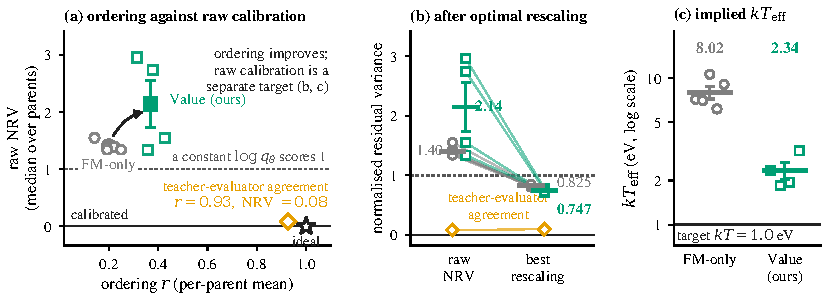
\includegraphics[width=\linewidth]{figures/out/fig4_calibration.pdf}
\end{center}
\caption{Archived readout results; likelihood labels in the plots refer to $\widehat\ell_\theta$, not a validated generator density. \textbf{Value supervision improves ordering before calibration.}
Same 93 held-out parents as \Cref{fig:ordering}, reference geometry dropped, GFN2-xTB evaluator;
five seeds for the flow-matching control, four for the value arm (open markers; filled marker or
rule the arm mean, bar its standard error over seeds). Metrics: ordering $r$ against raw
calibration $\mathrm{NRV} = \mathrm{Var}(\log q_\theta + E/kT)/\mathrm{Var}(E/kT)$ \textbf{(a)},
the optimally rescaled residual $\mathrm{NRV}_{\min}$ \textbf{(b)}, and the implied
$kT_{\mathrm{eff}}$ \textbf{(c)}. Three diagnostics move toward the Boltzmann-consistent regime:
$r$ rises from $0.200$ to $0.369$, $\mathrm{NRV}_{\min}$ falls from $0.825$ to $0.747$, and
$kT_{\mathrm{eff}}$ moves from $8.02$ to $2.34$~eV toward the $kT = 1.0$~eV target. Raw residual
variance --- the diagnostic most directly aligned with the objective as displayed --- remains a
separate unmet target: NRV rises from $1.402$ to $2.144$, past the $1$ that a constant
log-density scores, showing that errors in response magnitude and energy-unaligned variation
remain even as ordering improves. The value arm ($5/4/1$ launched / completed / diverged) is
conditional on completion. The orange marker is the teacher-evaluator agreement reference (not a
ceiling); panel detail and its derivation are in \Cref{app:figdetail}.}
\label{fig:calibration}
\end{figure}
